\chapter{Patterns' details}\label{appen:patterns}
In this appendix, we explain some technical aspects of the patterns of Chapter~\ref{chp:4} and expose some of their limitations.

%\section{Transversal vs longitudinal data}

\section{Patterns in depth}
\subsection{AFD}
The lognormal distribution could be validated by the fact that its support, spanning from zero to infinity, aligns with the natural constraints of any population. Contrarily, the gamma distribution does not contain $0$ in its support, making it difficult to interpret sampling errors. However, as noted in \cite{halley2002lognormality}, the Gaussian distribution is well-known for reproducing people's heights, which cannot be negative, despite being defined for all real numbers. \\

Regarding sampling errors, this pattern is sensitive to them. Both proposed distributions present fat tails, meaning that the probability density decreases much more slowly as we move away from the mean.  This implies that extreme events --a species being very rare or very abundant in a community-- are more likely to occur than in a Gaussian distribution. However, in real data, rare species/hashtags are usually underrepresented, creating a possible distorted pattern. \\

Precisely because of this sensitivity to sampling errors, the fluctuation distribution analysis has been carried out with the most abundant hashtag $h_m$ that appears consistently in every bin, which is defined as $\textrm{max}\{ \sum_{b=1}^B x_{hb}: h = 1,...,H \}$. %The distributions for the second and third most abundant hashtags are in Appendix's Figure X. 
We have chosen a hashtag that is present in all bins because if a hashtag is missing in one bin, it is not clear whether this absence is due to a sampling error. If a dataset has no hashtag appearing in every bin, we take the most abundant hashtag that appears in at least $70\%$ of the bins and we don't take those zero-abundance bins into account for computing the abundance distribution. \\


 The test decisions for the hypothesis that the data comes from a gamma, a Gaussian, or a lognormal distribution are done using the Lilliefors test at the $5\%$ significance level. All the distributions show a consistent unimodal shape, and the Gaussian distribution obtained superior performance. The gamma distribution is very versatile, in the sense that its shape varies greatly depending on the combination of the two parameters: from a monotonic decreasing function to an asymmetric unimodal. But the fact that the goodness of fit of the Gaussian distribution is better suggests that whichever mechanism is responsible for the variation in hashtags abundance, it consistently generates a unimodal distribution. Moreover, the probability that a gamma-distributed hashtag is exactly zero vanishes, which was a very strong assumption for hashtag dynamics. 
 

\subsection{Taylor's law} In our case, the variation is calculated over the bins in each dataset. The logarithm of the mean relative abundance is fitted as a linear regression $\log{\sigma_h} = a*\log{\overline{x}_h} + c$, with an expected slope of $a \leq2$. Hashtags with zero variance are not considered, as they only appear once in the whole dataset. Moreover, the fit improves if we set a threshold to the minimum percentage of bin absences a hashtag is allowed to take part in the fit. In particular, a $50\%$ coverage in Figures~\ref{fig:4:TAY}, \ref{chp:4:fig:Lego} and~\ref{fig:appen:LegoAux}. There are hashtags with very low relative abundances ($\overline{x}_h \ll 10^{-7}$), which tend to have a smaller-than-predicted variance. The effect of this threshold is to discard  these hashtags.\\

The sought-after exponent of $2$ may also arise from several other mechanisms than the ones cited in Chapter~\ref{chp:4}, mainly regarding sampling biases \cite{taylor1961aggregation}. But since we have also observed Taylor's law when it was calculated over bootstrapped data, these factors have been eliminated as potential explanations \cite{grilli2020macroecological}. By bootstrapped data, we mean when the bins are created in an alternative way, by randomly sampling them from the whole dataset with replacement $B$ times. This technique known as bootstrapping is commonly used to obtain better statistics of datasets without assuming any underlying mechanism for the creation of the data. \\

Finally, simple models with random demographic events in the dynamics of a population with four processes (birth, death, immigration, and emigration rates) can give rise to a power-law relationship between variance and mean abundance. The precise exponent and form of the relationship are set by the relative magnitude of the aforementioned ingredient processes and by the degree of  temporal and/or spatial heterogeneity \cite{anderson1982variability}.

\subsection{STAC} This distribution presents tails heavier than a Gaussian distribution, where the latter is  expected when the growth is affected by random processes. With heavy tails, short-term fluctuations can be large with a higher probability. The Laplace distribution of abundance variability is theorized to arise in populations with density-dependent birth and death rates, and with migration, which is a description that suits the dynamics of the online social network Twitter, and that it is compatible too with a gamma-distributed AFD.\\
 
 To obtain the average distribution $p(\lambda)$, we first calculate the distribution of short-term changes for each hashtag across all temporal bins. We then aggregate the distributions from all considered hashtags. We required, following the methods in \cite{ji2020macroecological}, a minimum mean relative abundance of  $10^{-3}$ and a $50\%$ of coverage among the bins. \\

For some datasets, the tails present points that are over the curve (Figure~\ref{fig:4:STAC}), so tails are even heavier than expected by a Laplace distribution. There are then hashtags that increase their abundance drastically, and also hashtags that decrease it with the same  harshness since the distributions are symmetric. We theorized that those hashtags are related to sudden discussions around the events, as the outlier points are not present in the random sampling.

\newpage
 \section{Estimate of parameters and statistical tests \label{appen:patterns:tests}}

 \begin{table}[h] 
\caption[$\,$ AFD: Estimated parameters and tests]{Estimated parameters across datasets for AFD. A $1$ in the test column means that Lilliefors or Chi-squared tests (T.) have rejected the null hypothesis at the $0.5\%$ significance level.}
\centering 
\begin{tabular}{c c c c c c} 
\hline 
Dataset &  $\beta_{h_m}$ & T. Gamma & T. LogNorm & T. Normal \\ \hline \hline
Mexican Elections & 3.70 & 1 & 1 & 1 \\ \hline 
Scotland Referendum & 2.20 & 1 & 1 & 1 \\ \hline 
Catalan Referendum & 1.37 & 1 & 0 & 1 \\ \hline 
St Patrick's Day & 84.64 & 1 & 1 & 1 \\ \hline 
Brexit & 13.20 & 1 & 0 & 1 \\ \hline 
UK random & 1.83 & 0 & 0 & 1 \\ \hline 
Ferguson Unrest & 4.33 & 1 & 1 & 0 \\ \hline 
Panama Papers & 6.74 & 1 & 0 & 1 \\ \hline 
Euro 2012 & 3.71 & 1 & 1 & 1 \\ \hline 
Nepal Earthquake & 28.75 & 1 & 0 & 1 \\ \hline 
Hurricane Sandy & 46.49 & 1 & 0 & 1 \\ \hline 
\end{tabular} 
\end{table} 

\begin{table}[h] 
\caption[$\,$ MAD: Estimated parameters and tests]{Estimated parameters across datasets for MAD. }
\centering
\begin{tabular}{c c c c } 
\hline 
Dataset &  $\mu$ & $\sigma$  \\ \hline \hline
Mexican Elections & -6.35 & 1.11   \\ \hline 
Scotland Referendum & -7.81 & 1.35   \\ \hline 
Catalan Referendum & -7.84 & 1.19   \\ \hline 
St Patrick's Day & -10.74 & 1.09  \\ \hline 
Brexit & -10.30 & 1.17  \\ \hline 
UK random & -8.54 & 0.73  \\ \hline 
Ferguson Unrest & -9.55 & 1.22  \\ \hline 
Panama Papers & -11.40 & 1.11  \\ \hline 
Euro 2012 & -12.01 & 1.27  \\ \hline 
Nepal Earthquake & -13.25 & 1.22  \\ \hline 
Hurricane Sandy & -12.85 & 1.13  \\ \hline 
\end{tabular} \label{tab:MAD}
\end{table} 

\begin{table}[t] 
\caption[$\,$ STAC: Estimated parameters]{Estimated parameters across datasets for STAC.}
\centering
\begin{tabular}{c c c c c} 
\hline 
Dataset & u & $\gamma$ & Cramér-Rao Bounds & $RMS$  \\ \hline \hline
Mexican Elections & -0.006 & 0.567 & 3.412e-05 & 0.504  \\ \hline 
Scotland Referendum & -0.044 & 0.564 & 2.074e-04 & 0.438  \\ \hline 
Catalan Referendum & -0.027 & 0.735 & 1.040e-04 & 0.339  \\ \hline 
St Patrick's Day & -0.010 & 0.437 & 5.056e-05 & 0.201  \\ \hline 
Brexit & 0.006 & 0.665 & 1.117e-04 & 0.240  \\ \hline 
UK random & -0.004 & 0.695 & 4.102e-05 & 0.216  \\ \hline 
Ferguson Unrest & -0.001 & 0.509 & 2.023e-05 & 0.239  \\ \hline 
Panama Papers & 0.004 & 0.800 & 1.489e-04 & 0.118  \\ \hline 
Euro 2012 & -0.014 & 0.728 & 3.019e-05 & 0.053  \\ \hline 
Nepal Earthquake & 0.001 & 0.499 & 2.190e-05 & 0.133  \\ \hline 
Hurricane Sandy & -0.005 & 0.375 & 1.293e-05 & 0.246  \\ \hline 
\end{tabular} \label{tab:STAC}
\end{table} 

 \newpage
\section{Theoretical prediction of the multinomial random sampling model \label{appen:patterns:eqs}}
 Multinomial sampling allows us to create analytical null predictions that are not influenced by any particular system dynamics or external factors. The  resampled bins are not time-correlated since the extractions are independent, nor are they correlated in any other complex way following functional or structural properties of the empirical dataset from which they are sampled. Independent selection also makes the model unbiased, so the sample is not systematically skewed in any particular direction. All this implies that the abundances of the new bins are more likely to be similar to the frequencies from which they were drawn, making the multinomial random sampling a useful tool for testing how patterns emerge.\\

To obtain the theoretical exponent for Talyor's law, we get the analytical relation between the expected abundance of hashtags and their variance. If the abundance is drawn by a multinomial distribution, this relation is linear:
\begin{equation}
    E(n_{hb}) \sim Var(n_{hb})
\end{equation}
Taylor's law, however, evaluates relative abundances, $x_{hb} = n_{hb}/N_b$. One can easily compute the expected relative abundances and their variances from $ n_{hb}$ by adding them over the bins. Since they are independent random variables, the linear relationship is conserved by the central limit theorem. We should then find an exponent of one instead of two.\\

Regarding the MAD, if the number of bins $B$ is high enough, we expect to recover the actual frequencies from which we have drawn the hashtags. \\

For the approximation of the AFD, let's first assume that the size of each  bin $N_b$ is equal for all random samples. If we focus on one hashtag, the probability of drawing that hashtag is one minus the probability of drawing any other hashtag. Therefore, the probability that a hashtag has a certain abundance is given by the binomial distribution $\textrm{B}(N_b,f_h)$, because the number of appearances of the hashtag in a sequence of $N_b$ independent trials is given by that yes-no question (whether that hashtags have been chosen or a different hashtag has been chosen instead). The probability of hashtag $h$ appearing in $n$ posts is given by:
\begin{equation}
    \rho'_h(n)  = {N_b\choose n} f_h^n (1-f_h)^{N_b-n} 
\end{equation}
Relative abundances are just abundances divided by a constant, and the binomial distribution still holds. In our situation, each bin has a different size and the AFD is not a binomial distribution but reflects the fact that some bins have a higher number of hashtags than expected because they correspond to periods of high activity. Remember that some datasets are collected around one or several events with their corresponding burst in posting. The most abundant hashtag is expected to be part of the event and will consequently have a high use frequency. \\

In Figure~\ref{fig:appen:LegoAux}, we have plotted the patterns obtained by multinomial random sampling and confronted them with the expected theoretical predictions.

\begin{figure}[t]
    \centering
    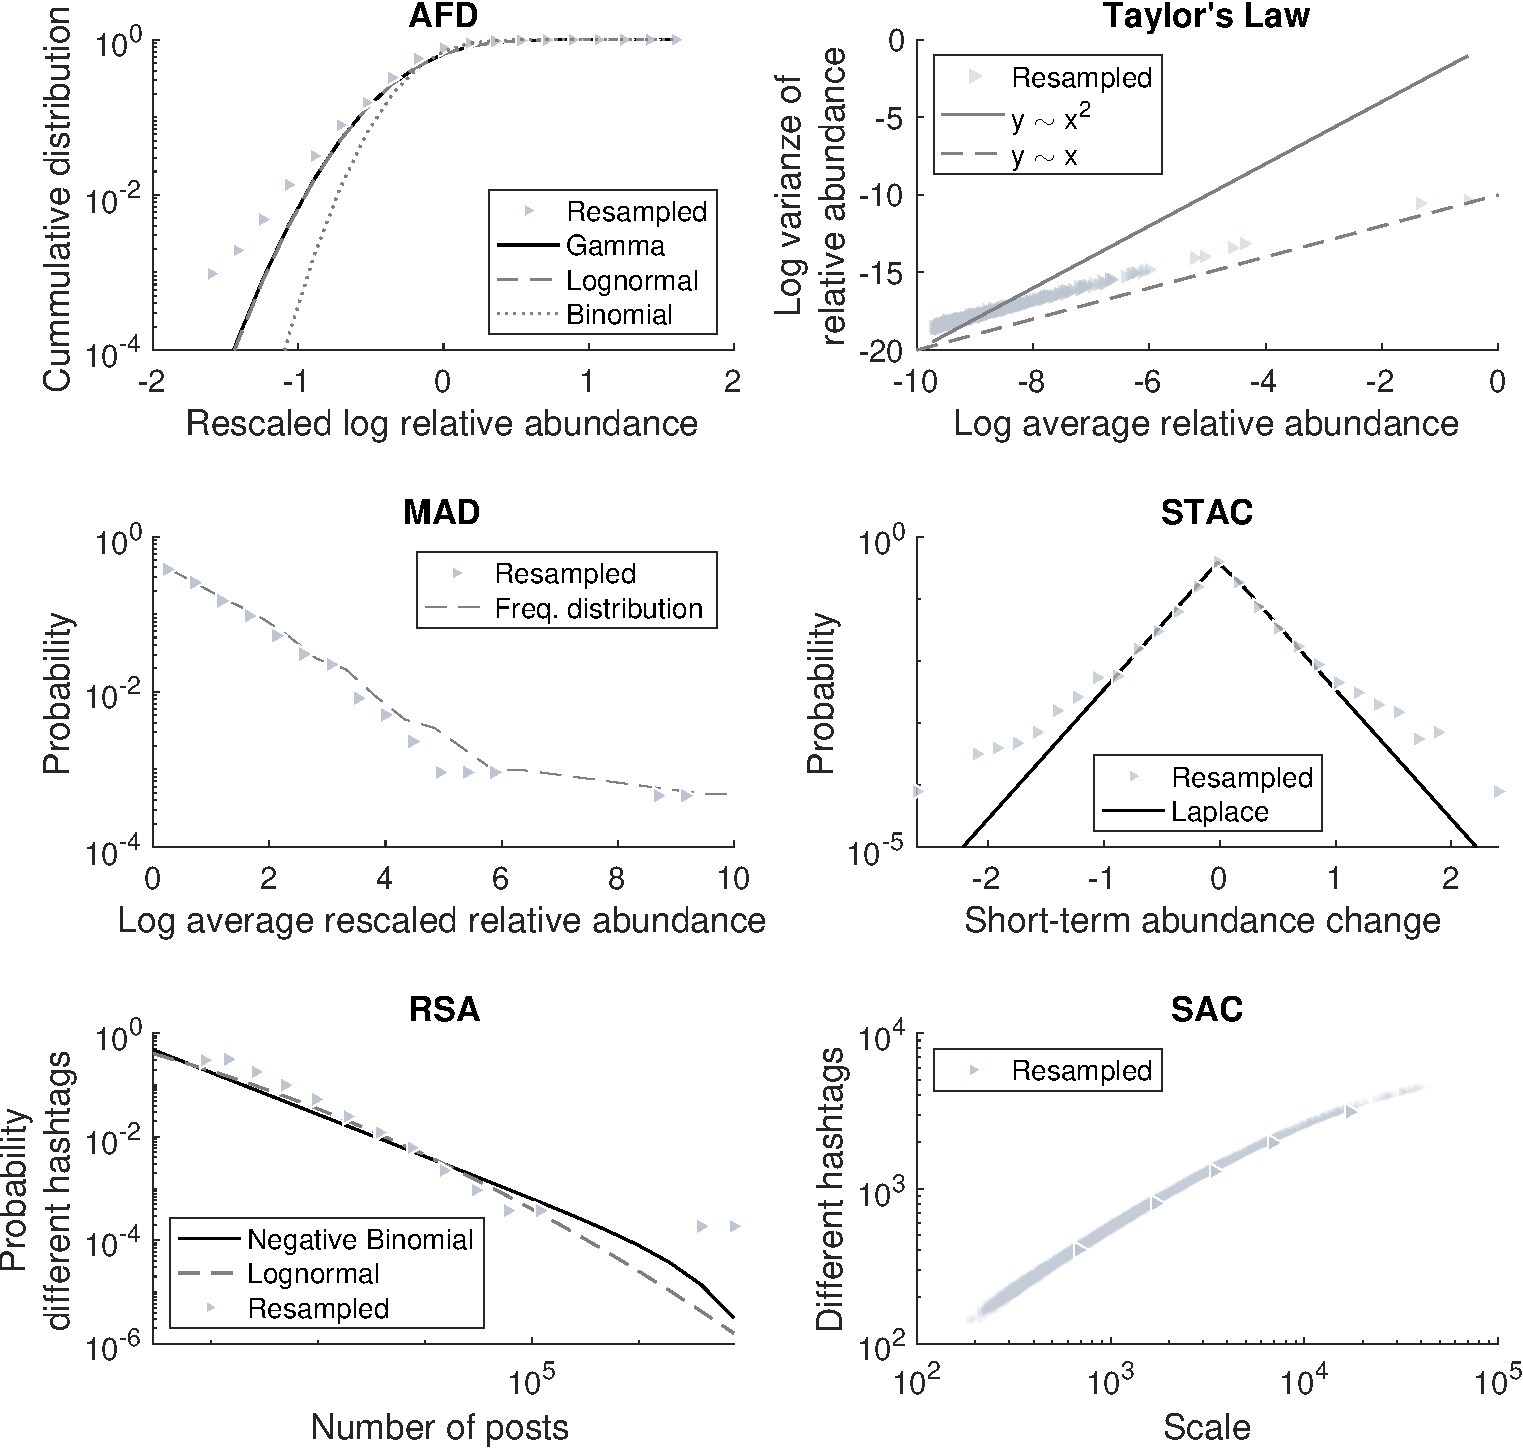
\includegraphics[width=\textwidth]{figures/chp4/Figure_Lego_gray.pdf}
    \caption[Macropatterns by multinomial random sampling]{Macropatterns (gray dots) obtained by multinomial random sampling of the largest dataset (Hurricane Sandy) and their fits to theoretical predictions. The dots correspond to one of the gray lines of Figure~\ref{chp:4:fig:Lego}.}
    \label{fig:appen:LegoAux}
\end{figure}

%The short-term abundance change involves the ratio between two relative abundances. We already know that the abundances are binomially distributed from the derivation of the theoretical AFD. Let these distributions be $\textrm{B}(V,f_h)$ and $\textrm{B}(N'_b,f_h)$, and the quotient $\Lambda_{hb} =\frac{n_{hb+1}}{n_{hb}}$. Assuming there is no temporal correlation, $\log(\Lambda_{hb})$ is approximately normally distributed with mean $\log{\frac{f_h}{f_h}} = 0$ and variance $\frac{(f_h^{-1}-1)(N'_b+V)}{N'_bV}$ \cite{katz1978obtaining}. If we constrain ourselves to the case of constant bin size $N'_b = V$, we obtain that the probability of a certain change aggregating over all hashtags is:
%\begin{equation}
 %  p(\Lambda) \sim  \mathcal{N}\left(0,\sqrt{\frac{2}%{V}\sum^H_{h = 1} f_h^{-1}-1} \right)
%\end{equation}
